The Singleton Interface Method is based on consolidating all parameters and customizations into a single
method definition.
Typically, some parameters are nullable due to the existence of a default value, employed in case of a null value
(as specified in the business logic) or when the parameter is not used in combination with others.
For instance, the maximum response time is not utilized in the context of the Leave Group message.
This approach represents the simplest way to design an API\@.

Figure~\ref{fig:sing_write_igmp_packet} illustrates the activity diagram featuring the interface definition
of the method for writing an IGMPv2 packet into the output stream.
All parameters, including the message type, are condensed into a singular interface method.
Only the parameters \textit{igmpType} and \textit{outputStream} are mandatory; others may contain \textit{null} values
depending on the \textit{igmpType} parameter's value.

\begin{figure}[!htb]
    \centering
    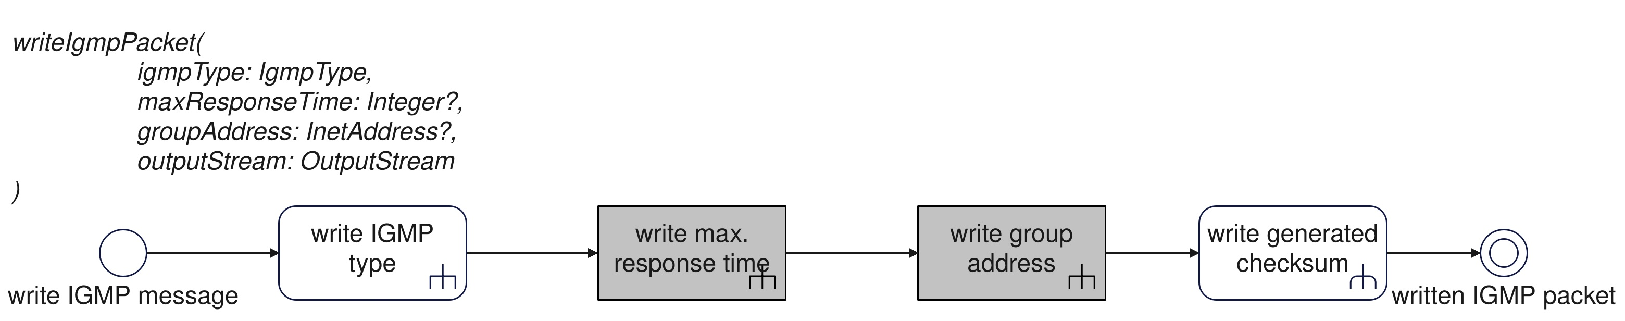
\includegraphics[width=1.0
    \textwidth]{sing_write_igmp_packet}
    \caption{Singleton Interface Method: Writing IGMP packet to output stream}
    \label{fig:sing_write_igmp_packet}
\end{figure}

The activity diagram also encompasses more intricate activities, such as writing the maximum response time
and group address, which must be broken down into smaller models.
For example, Figure~\ref{fig:sing_write_max_response_time} presents the content of the
\textit{write maximum response time} activity.
As the entire logic is implemented under a common interface method, the business logic involves numerous branches,
including conditional statements to handle invalid combinations of input parameters.

\begin{figure}[!htb]
    \centering
    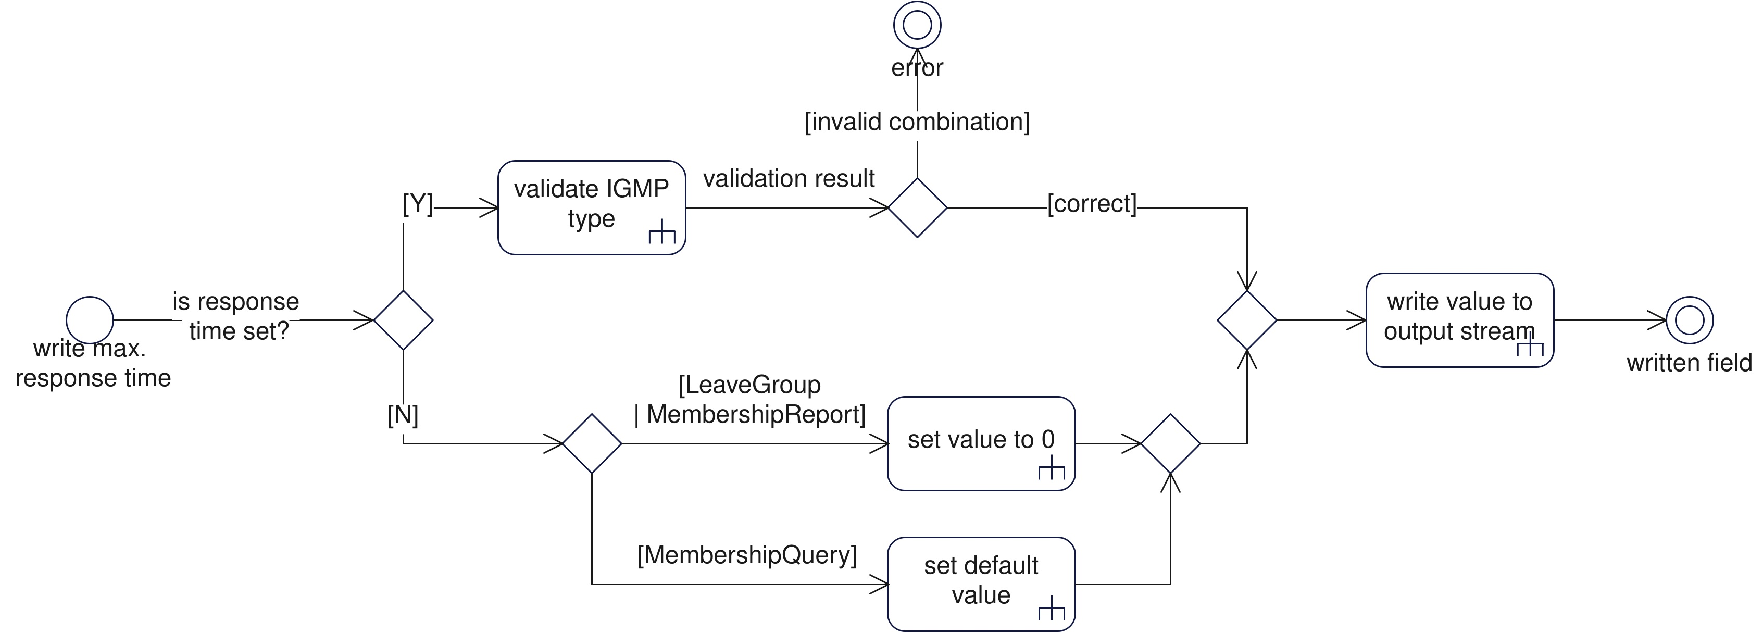
\includegraphics[width=1.0
    \textwidth]{sing_write_max_response_time}
    \caption{Singleton Interface Method: Writing maximum response time}
    \label{fig:sing_write_max_response_time}
\end{figure}

Benefits of the Singleton Interface Method:

\begin{itemize}
    \item
    Definition of the interface is straightforward and simple, eliminating the need for additional software entities.
    \item
    Serving as a single point of contact for the API client can be advantageous in certain cases.
    For instance, the client may act as an additional proxy layer on top of the API,
    receiving all necessary parameters from other components in the system.
    Further layer decomposition would introduce unnecessary complexity in the proxy layer,
    requiring the correct method to be called based on specific conditions.
\end{itemize}

Drawbacks of the Singleton Interface Method:

\begin{itemize}
    \item Occurrence of God Classes/Functions:
    The implementation of all logic within a single method often results in complexity and extensive branching.
    Understanding and maintaining such logic can be challenging in the long term.
    The concepts of Long Methods and Long Classes were introduced by Martin Fowler in the book Refactoring:
    Improving the Design of Existing Code~\cite[Chapter~3]{fowler1999refactoring}.
    While this book doesn't explicitly use the term God Classes it introduces the idea of code smells and provides
    guidance on improving the design of code, which includes avoiding the creation of large, monolithic classes.
    Over time, as the software development community has grown and evolved, the term God Class has become more
    prevalent.
    \item Difficulty in API Evolution:
    Adapting the API to support additional packet fields, as seen in the case of IGMPv3~\cite{rfc3376},
    necessitates altering the interface method signature and updating all clients utilizing it.
    \item Nullable parameters:
    The presence of nullable parameters, dependent on the IGMP message type, requires additional logic
    in the implementation to handle invalid parameter combinations.
    Clients must be aware of valid combinations, and default values overriding null values may not be transparent
    to clients unless explicitly documented.
    \item Error-prone long parameter lists:
    In the absence of support for named parameters in the chosen technology, a long list of parameters becomes
    error-prone as clients must be mindful of the correct ordering.
    \item Violation of the Single Responsibility Principle (SRP):
    Such methods tend to accumulate responsibilities over time, violating the SRP by encompassing more than one
    distinct responsibility.
    SRP was described by Robert C. Martin in the book Agile software development: principles, patterns,
    and practices~\cite[Chapter~8]{martin2003agile}.
\end{itemize}

Common use-cases of the Singleton Interface Method:

\begin{itemize}
    \item Stable API with limited change expectations:
    The method is suitable for a stable API not anticipated to undergo significant changes in the future.
    It works well when there is a single behavior implemented by the service without customizations or subtypes.
    \item Simple services or utility functions:
    The method is appropriate for simple services or utility functions with a small number of non-null parameters,
    where complexity and branching are minimal.
\end{itemize}
